% This document is compiled using pdfLaTeX
% You can switch XeLaTeX/pdfLaTeX/LaTeX/LuaLaTeX in Settings

\documentclass{article}
% \usepackage[utf8]{inputenc}
\usepackage{graphicx}
\usepackage{float}
\usepackage{amssymb}
\usepackage{amsmath}

\title{Assignment 3}
\author{221300079 Juntong Wang}
\date{\today}
    %\begin{figure}[H]
    %    \centering
    %    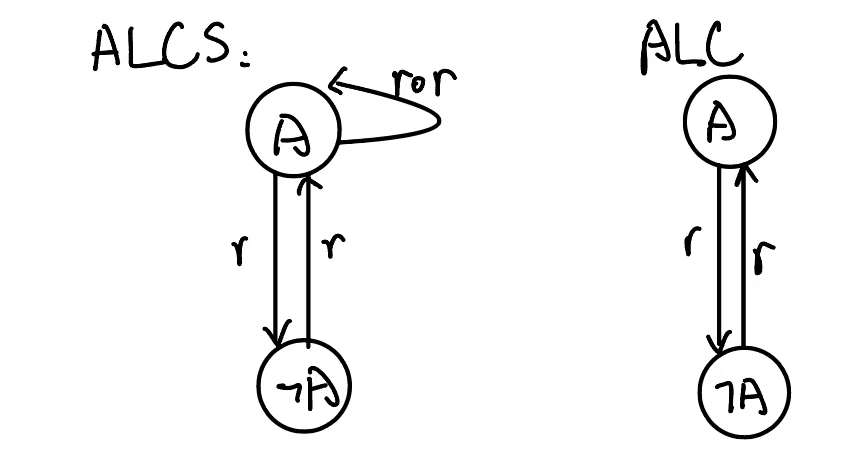
\includegraphics[width=1\textwidth]{4.png}\\
    %    \caption{Unraveling graph}
    %    \label{fig:Unraveling}
    %\end{figure}  

\begin{document}

	\maketitle

	\section{Question 1}
    \begin{itemize}
        \item Apply the Tableau algorithm $\textsf{consistent}(\mathcal{A})$ to the following ABox:
        \begin{center}
        $\mathcal{A}=\{(b,a):r, (a,b):r, (a,c):s, (c,b):s, a:\exists s.A, b:\forall r.((\forall s.\neg A)\sqcup(\exists r.B)), c:\forall s.(B\sqcap(\forall s.\bot))\}$.
        \end{center}If $\mathcal{A}$ is consistent, draw the model generated by the algorithm.
    \end{itemize}
    \textbf{Here is the answer:}\\
    If we want to generate the model by Tableau algorithm,the only thing we need to do is use the expansion rule to expand it till to be the complete and clash free model:\\
    Here is the way to expand it:\\
    step 1.$\exists \ rule$:
    \[
        A_1 = A  \cup \{(a,d) : s , d : A\}
    \]
    step 2:$\forall \ rule$:
    \[
        A_2 = A_1 \cup \{a : (\forall s.\neg A) \sqcup (\exists r .B)\}  
    \]
    For the min space of Tableau algorithm, we in the end to use the or rule to solve it.\\
    step 3:$\forall \ rule$:
    \[
        A_3 = A_2 \cup \{b : B \sqcap (\forall s .\perp )\}  
    \]
    step 4:$\sqcap \ rule$:
    \[
        A_4 = A_3 \cup \{b:B , b: \forall s. \perp\}  
    \]
    for this $A_4$ there is no rule to expand it, so we goto expand the formula in $A_2$,
    we firstly choose the first part of or rule:\\
    step 5:$\sqcup \ rule \ + \ \forall \ rule$:
    \[
        A_5 = A_4 \cup \{a: \forall s .\neg A\} 
    \]   
    \[
        A_6 = A_5 \cup \{c: \neg A,d : \neg A\}  
    \]
    But this is contradict to the expand result in $A_1$, so we try another part:\\
    step 6:$\sqcup \ rule \ + \ \exists \ rule$:
    \[
        A_5' = A_4 \cup \{a: \exists r .B\}
    \]
    And there is no element fit for the rules, so the model now is complete and clash free.And the model generate drawing is followed:\\
    \begin{figure}[H]
        \centering
        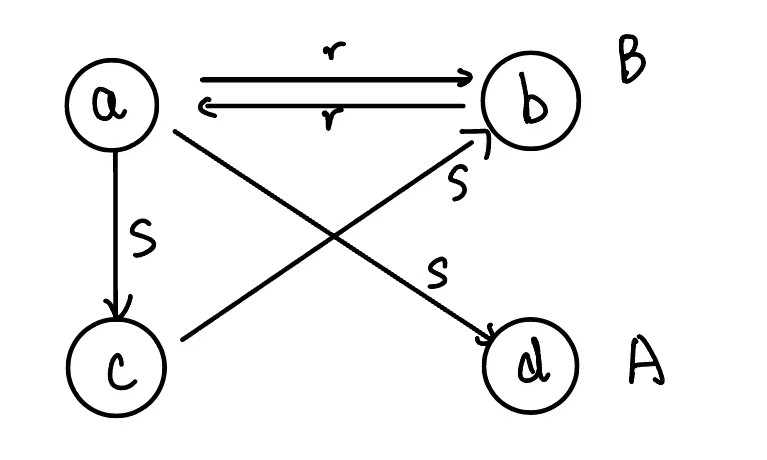
\includegraphics[width=1\textwidth]{1.png}\\
        \caption{expand model graph}
        \label{fig:expand model graph}
    \end{figure}  

    \section{Question 2}
    We consider an $\mathcal{ALC}$ TBox $\mathcal{T}$ consisting only of the following two kinds of axioms:
    \begin{itemize}
        \item  role inclusions of the form $r\sqsubseteq s$, and
        \item role disjointness constraints of the form $\textsf{disjoint}(r,s)$.
    \end{itemize}where $r$ and $s$ are role names. An interpretation $\mathcal{I}$ satisfies these axioms if
    \begin{itemize}
        \item  $r^{\mathcal{I}}\subseteq s^{\mathcal{I}}$, and
        \item $r^{\mathcal{I}}\cap s^{\mathcal{I}}=\emptyset$, respectively.
    \end{itemize}
    Modify the Tableau algorithm $\textsf{consistent}(\mathcal{A})$ to decide the consistency of $(\mathcal{T},\mathcal{A})$, where $\mathcal{A}$ is an ABox and $\mathcal{T}$ a TBox containing only role inclusions and role disjointness constraints. Show that the algorithm remains terminating, sound, and complete.\\
    \textbf{Here is the answer:}\\
    First we need to know that the inclusion means  $r^{\mathcal{I}}\subseteq s^{\mathcal{I}}$,but which r and s are disjoint, this means we have:
    $\{(a,b): r,(a,b): s,r\ and\ s\ \in A\},\{disjoint(a,b)\}$,so we could add an rule of inclusion:\\
    Rule of inclusion:\\ 
    Conditions: A contains $(a,b):r,r\in A$,$r \subseteq s$,and $(a,b):s,s \notin A$\\
    Actions:  $A'$ $\rightarrow$ $A \cup \{(a,b):s\}$
    Then we could start our proof:\\
    \textbf{Termination:}\\
    As the proof in class, we need to proof the rule of inclusion is bounded.So we assume size of C is less than m.
    In the proof without Tbox we have individual bound $size(c) \leq m$,so if individual is bounded,also the number of assertion is bounded,
    because the inclusion rule is not to expand the individual,so the use of inclusion rule is bounded.And also, the depth will not depend on the 
    new inclusion rule, because the new inclusion will not increase the depth of the whole model, so the depth is bounded. In all, all the restrictions 
    are bounded, so proved.\\
    \textbf{Soundness:}\\
    For the first,we need to prove the interpretation I and model A' is complete and clash free:\\
    For every disjoint (r,s), if $r^I \cap s ^I \neq \emptyset$, so this means there exists $(a,b):r,(a,b):s,which\ r \in A,s\in A$,so this is 
    contradict to the definition of complete and clash free A',so all the rules of disjoint is ok\\
    For the second, we need to do inductive:\\
    If $r \sqsubseteq s$,so we assume a and b: $(a,b):r$,so we get $(a,b):s$,but the inclusion rule says:$(a,b):r\in A, (a,b):s\notin A$,so this is contradict, so proof.\\
    \textbf{completeness:}\\
    If we have a model T,for $(a,b):r\in A$, because of the $r \sqsubseteq s$ fit for the model T,so we get the interpretation I, for $r^I \subseteq s^I$, so we
    get $(a,b)\in s^I$, so there exists at least one A' which means $A' \in exp(A,inclusion-rule,(a,b):r),r\in A$,$r \subseteq s$,and $(a,b):s,s \notin A$,so proved.

    \section{Question 3}
    Let $\mathcal{T}$ be an acyclic TBox in NNF. $\mathcal{T}^{\sqsubseteq}$ is obtained from $\mathcal{T}$ by replacing each concept definition $A\equiv C$ with the concept inclusion $A\sqsubseteq C$.
    \begin{itemize}
        \item[-] Prove that every concept name is satisfiable w.r.t.\ $\mathcal{T}$ iff it is satisfiable w.r.t.\ $\mathcal{T}^{\sqsubseteq}$. Does this also hold for the acyclic TBox $\{A\equiv C\sqcap\neg B, B\equiv P, C\equiv P\}$?
    \end{itemize}
    \textbf{Here is the answer:}\\
    $\Rightarrow$:\\
    We know that A $\equiv$ C is equal to $A \sqsubseteq C,C \sqsubseteq A$, so the $T^{\sqsubseteq}$ is the subset of it $T^{\sqsubseteq} \sqsubseteq T$, so according to lemma 2.5 we get the model of 
    $model\ T \sqsubseteq model\ T^{\sqsubseteq}$, so this means every concept name for T is satisfiable for $T^{\sqsubseteq}$\\
    $\Leftarrow$:\\ 
    To prove this, we do a little expand on the five rules to fit and explain why the example seems contradict to the Tbox we need to prove.\\
    Firstly, there are some differences between the primitive concept and complex concept.We could find that in the example below:\\
    \[
        \{A\equiv C\sqcap\neg B, B\equiv P, C\equiv P\}
    \]
    We could find that preciesly the concept B is not in the NNF we need.It is not in the most simple form, so to prove the are equal, we need to do some operation 
    on the 5 operators.\\
    We assume there is an interpretation I,and concept name $A_1,A_2,C_1,C_2,D_1,D_2$ and $D_1 = D_2$\\
    1.For the negative form:\\
    $A_1 \equiv \neg C_1,A_2 \sqsubseteq \neg C_2$ we could get $A_1^I = \neg C_1^I,A_2^I \subseteq \neg C_2^I$, and also we have:$C_1 \equiv C_1,C_2 \equiv D_2,D_1 = D_2$,so we get
    $C_2^I \subseteq C_1^I$,so we could get $A_1^I \subseteq A_2^I$.through this form we could see that the space is bigger than we think, the correct form of this we need is $A_2^I \subseteq A_1^I$.\\
    2.For or/ and form:\\
    The same proof as above, but we get:$A_2^I \subseteq A_1^I$.\\
    3.For exists/ forall form:\\
    The same proof as above, but we get:$A_2^I \subseteq A_1^I$.\\
    So for this problem, we only need to do a more nnf for negative form, that is:\\
    \textbf{If the complex concept in the Tbox with negative operator, we need to replace it with its primitive form, and use the NNF to let it into the most simple form.}\\
    So after we do this nnf in the Tbox, there no negative operator ahead the complex concept.Thus, we could prove that:$A \sqsubseteq C$ could prove $A \equiv C$.\\
    So after the initial operation:for the acyclic Tbox, we change some steps of unfolding rules,and in order to unraveling the tree property.Because all the negative form operator are pushed into the leave node.We could use tree in safe\\ 
    \textbf{Firstly} we need to know what is the acyclic Tbox, this means:(1).no definitions like $A\equiv C,A\equiv D$.(2).no cycle definition like $A_{i+1} in\ C_i,A_1 in\ C_n$\\
    \textbf{Secondly}, we could find the tree structure which is perfectly fit for the requirement of the Tbox.And we could find a simply way to expand the tree, that is:
    \[
        A = C,C = D \sqcup E \ \ A = D \sqcup E,\ \ A \sqsubseteq D \sqcup E    
    \]
    which D and E is the child of C,C is the node of A and C have some inclusions.\\
    \textbf{Third},we have the theorem said that the for the ontology the model of it is infinite,so we define a tree in this form,\textbf{K level tree} which means we have a tree like this:\\
    In the 1 to k level of the expansion tree, we define the things like $A_i \equiv C_i$\\
    In the k+1 level to n of the expansion tree, we define the tree in the inclusion form $A_i \sqsubseteq C_i$\\
    So now if we want to prove the every concept name is satisfiable for $T^{\sqsubseteq}$ also fit for $T$,there is to find an interpretation $I_k$ which fit for the model $T^{\sqsubseteq}$ must be the model of T.\\
    \textbf{Fourth},we use the math induction to prove it.\\
    Base: i = 1, always holds for both two situation\\
    I.H:i = k-1 also fit.\\
    I.S:if we want to prove $A \equiv C$, we alread have $A \sqsubseteq C$, we need to prove $C \sqsubseteq A$,to prove this , we assume $A_k = A_{k+1} \cup A_x$, so according to the structure of a tree we have x must bigger than 
    k-1, but if x = k , we proved, if x not equal to k, we could do expand to $A_k$, so we will have cycle in the tree, this is not fit for the definition of it. So inductive finished!\\
    \textbf{Finally},we have proved that this is also holds for it.\\



    However, this is not hold for the the acyclic TBox $\{A\equiv C\sqcap\neg B, B\equiv P, C\equiv P\}$.\\
    Because for Tbox,we have $A \equiv C\sqcap\neg B = C\sqcap\Delta /B, B \equiv P,C\equiv P$,so we bring into the B and C we get the A is emptyset, so this is not satisfiable.\\
    But for the $T^{\sqsubseteq}$Box, this is not satisfiable, because if the domain is \{a,b,c\},A is \{a\},B is \{b\}, C is \{a,c\},P equal to domain, we get all the restriction is satisfiable.\\
    So this Question is not satisfiable for acyclic TBox.

    \section{Question 4}
    Let $E$ be an ALC-concept. By $\#E$ we denote the number of occurrences of the constructors $\sqcap$, $\sqcup$, $\exists$, $\forall$ in $E$. The multiset $M(E)$ contains, for each occurrence of a subconcept of the form $\neg F$ in $E$, the number $\#F$.
    
    \begin{itemize}
        \item[-] Following this representation, prove that exhaustively applying the transformations below to an ALC concept always terminates, regardless of the order of rule application:
        \begin{align*}
            \neg(E\sqcap F)&\leadsto\neg\neg\neg E\sqcup\neg\neg\neg F\\
            \neg(E\sqcup F)&\leadsto\neg\neg\neg E\sqcap\neg\neg\neg F\\
            \neg\neg E&\leadsto E\\
            \neg(\exists r.E)&\leadsto\forall r.\neg E\\
            \neg(\forall r.E)&\leadsto\exists r.\neg E
        \end{align*}
    \end{itemize}
    \textbf{Here is the answer:}\\
    To solve this question, we use the structured induction for the 5 applications:\\
    As we need to prove it terminates:\\
    (1).For the first rule:\\
    $M(\neg (E \sqcap F)) = \{\#(E \sqcap F)\}$\\
    $M(\neg\neg\neg E\sqcup\neg\neg\neg F) =\{\#\neg\neg E,\#\neg\neg F,\#\neg E,\#\neg F,\# E,\# F\}$\\
    So the new $M(C') = M(C) / \{\#(E \sqcap F)\} \cup \{\#\neg\neg E,\#\neg\neg F,\#\neg E,\#\neg F,\# E,\# F\}$.So it could be convert to one of this small form\\
    (2).For the second rule:\\
    $M(\neg (E \sqcup F)) = \{\#(E \sqcup F)\}$\\
    $M(\neg\neg\neg E\sqcap\neg\neg\neg F) =  \{\#\neg\neg E,\#\neg\neg F,\#\neg E,\#\neg F,\# E,\# F\}$\\
    So the new $M(C') = M(C) / \{\#(E \sqcup F)\} \cup \{\#\neg\neg E,\#\neg\neg F,\#\neg E,\#\neg F,\# E,\# F\}$.So it could be convert to one of this small form\\
    (3).For the third rule:\\
    $M(\neg\neg E) = \{\#(\neg E), \#(E)\}$\\
    $M(E) = 1$\\
    So the new $M(C') = M(C) / \{\#(\neg E), \#(E)\}$.So it could be convert to one of this form.or I say this form is the smallest.\\
    (4).For the fourth rule:\\
    $M(\neg (\exists r.E)) =\{\# \exists r.E\}$\\
    $M(\forall r.\neg E) =\{\#(\forall r.\neg E, \# E)\}$\\
    So the new $M(C') = M(C) / \{\# \exists r.E\} \cup  \{\#(\forall r.\neg E, \# E)\}$.So it could be convert to one of this small form.\\
    (5).For the fifth rule:\\
    $M(\neg (\forall r.E)) =\{\# \forall r.E\}$\\
    $M(\exists r.\neg E) =\{\#(\exists r.\neg E, \# E)\}$\\
    So the new $M(C') = M(C) / \{\# \forall r.E\} \cup  \{\#(\exists r.\neg E, \# E)\}$.So it could be convert to one of this small form.\\
    As it is shwon above, all the 5 applications could be convert to small and easy form,this calculate form will decrease, so his means all the situation could be terminates in the end.So proved.\\

    \section{Question 5}
    We consider the Tableau algorithm $\textsf{consistent}(\mathcal{T},\mathcal{A})$ for acyclic TBoxes $\mathcal{T}$, which is obtained from $\textsf{consistent}(\mathcal{A})$ by adding the $\equiv_{1}$-rule and the $\equiv_{2}$-rule for unfolding $\mathcal{T}$.
    \begin{itemize}
        \item[-] Prove that $\textsf{consistent}(\mathcal{T},\mathcal{A})$ is a decision procedure for the consistency of $\mathcal{ALC}$-knowledge bases with acyclic TBoxes.
    \end{itemize}
    \textbf{Here is the answer:}\\
    To prove the consistency in this acyclic Tbox, in abox with acyclic Tbox, there is an operation to convert the acyclic Tbox 
    into Abox without Tbox by the unfolding, it says:\\
    The $\equiv_1 -rule$:\\
    Condition:$a:A\in \mathcal{A} ,A\equiv C\in \mathcal{T},and\ a:C \notin \mathcal{A}$,do Action:$A\rightarrow \mathcal{A}\cup \{a:C\}$\\
    The $\equiv_2 -rule$:\\
    Condition:$a:\neg A\in \mathcal{A} ,A\equiv C\in \mathcal{T},and\ a:\neg C \notin \mathcal{A}$,do Action:$A\rightarrow \mathcal{A}\cup \{a:\neg C\}$\\
    The only thing we need do is to prove these two rules added in Abox will satisfiable Termination,Soundness and completeness\\
    \textbf{Termination}\\
    To prove the Termination, firstly, two of the rules will not decrease the assertion number in the Abox,and we know if there exists a $|sub(A)| \geq size(A) = m$,and 
    all the $\equiv$ forms are restrect by the size of model, so the use of the two rules are limited.And also for two rules, they never add new element into the subset, so
    the size is bounded by the m.Also the depth is bounded by $\exists\ and\ \forall$, so the size is decreased,it will reach Termination.\
    \textbf{Soundness}\\
    Also use the expansion rules in the proof of Abox without Tbox, so first the new interpretation I is satisfiable because the interpretation I's domain is not emptyset
    and all the $a^I,A^I,r^I$ is in the domain. So here is a new model called A',we need to prove $C\equiv D$ the $a:D$ is in the A' by induction:\\
    A' is clash free, so $a:C$ is also in A', $C\equiv D$, so $a:D$is in A', but $a:D$is not in  A, so the expand is soundness and clash free.this is also holds for 
    rule 2, so the soundness is proved.\\
    \textbf{completeness}\\
    First,prove that add the rule 1 will not cause clash,if $a:A \in \mathcal{A}$,$A\equiv C\in \mathcal{T},and\ a:C \notin \mathcal{A}$,this means the $a^I\in A^I$and $a^I \notin C^I$,but the $A\equiv C$, to
    not cause the clash, there exists an A'$A' \in exp(A,\equiv_1-rule, a:A\in \mathcal{A}, a:C\mathcal{A})$,so the rule 1 will not cause the clash. Also the same way to prove the rule 2.So the completeness proved.\\

    \section{Question 6}
    \begin{itemize}
        \item[-] Use the Tableau algorithm $\textsf{consistent}(\mathcal{T},\mathcal{A})$ for acyclic TBoxes to determine whether the subsumption
        \[\neg(\forall r.A)\sqcap\forall r.C\sqsubseteq_{\mathcal{T}}\forall r.E\]holds w.r.t.\ the acyclic TBox
        \[\mathcal{T}=\{C\equiv(\exists r.\neg B)\sqcap\neg A, D\equiv\exists r.B, E\equiv\neg(\exists r.A)\sqcap\exists r.D\}.\]
    \end{itemize}
    \textbf{Here is the answer:}\\
    Firstly,reduction to satisfiability:\\
    \[
        \neg(\forall r.A)\sqcap\forall r.C\cup \neg\forall r.E
    \]
    Then:reduction to consistency:\\
    \[
        \{a:(\neg(\forall r.A)\sqcap\forall r.C\sqcup \neg\forall r.E)\}  
    \]  
    Expansions:$\sqcap\ rule$\\
    \[
        \{a:\exists r.\neg A,a:\forall r.C,a:\exists r.\neg E\}  
    \]
    exists rule:\\
    \[
        \{(a,d):r,d:\neg A, (a,d_1):r,d_1:\neg E,a:\forall r.C\}  
    \]
    forall rule:\\
    \[
        \{(a,d):r,(a,d_1):r,d:C,d:\neg A,d_1:C,d_1:\neg E, \}  
    \]
    and for Tbox,use the rule 1 and rule 2:\\
    (1)for d:C:\\
    \[
        d:(\exists r.\neg B)\sqcap\neg A
    \]
    cap rule:\\
    \[
        d:\exists r.\neg B,d:\neg A
    \]
    exists rule:\\
    \[
        (d,d'):r,d':\neg B
    \]
    so the abox:\\
    \[
        \{(a,d):r,(a,d_1):r,(d,d'):r,d:C,d:\neg A,d_1:C,d_1:\neg E,d':\neg B \}  
    \]
    (2)for $d_1:C$:\\
    \[
        d_1:(\exists r.\neg B)\sqcap\neg A
    \]
    cap rule:\\
    \[
        d_1:\exists r.\neg B,d:\neg A
    \] 
    exists rule:\\
    \[
        (d,d_1'):r,d_1':\neg B
    \]
    so the abox:\\
    \[
        \{(a,d):r,(a,d_1):r,(d,d'):r,(d,d_1'):r,d:C,d:\neg A,d_1:C,d_1:\neg E,d':\neg B,d_1':\neg B \}  
    \]
    (3)for $d_1:\neg E$:\\
    \[
        d_1:\exists r.A \sqcup \forall r. \neg D  
    \]
    cup rule:we assume the first part\\
    \[
        d_1 :\exists r.A
    \]
    exists rule:\\
    \[
        (d_1,d_1''):r,d_1'':A
    \]
    So the abox:\\
    \[
        \{(a,d):r,(a,d_1):r,(d,d'):r,(d,d_1'):r,(d_1,d_1''):r,d:C,d:\neg A,d_1:C,d_1:\neg E,d':\neg B,d_1':\neg B,d_1'':A \}  
    \]
    So there is no clash,so this is consistent.\\

    \section{Question 7}
    We consider a different form of blocking, which allows individuals to be blocked by individuals who are not necessarily their ancestors, known as anywhere blocking. This approach employs an individual $a$'s age, denoted as $\textsf{age}(a)$, to determine the blocking relationship, instead of relying on the ancestor relation.\\
    The $\textsf{age}$ of an individual is defined as $0$ for individuals that occur in the input ABox $\mathcal{A}$, while a new individual generated by the $n$th application of the $\exists$-rule is assigned an age of $n$. This approach expands the scope of blocking beyond the ancestor relation, enabling individuals to be blocked based on their age, which could result in more effective blocking in certain situations.\\
    Let $\mathcal{A}^{\prime}$ be an ABox obtained by applying the Tableau rules of $\textsf{consistent}(\mathcal{T}, \mathcal{A})$ for general TBoxes. A tree individual $b$ is anywhere blocked by an individual $a$ in $\mathcal{A}^{\prime}$ if
    \begin{itemize}
        \item[$\bullet$] $\textsf{con}_{\mathcal{A}^{\prime}}(b)\subseteq\textsf{con}_{\mathcal{A}^{\prime}}(a)$,
        \item[$\bullet$] $\textsf{age}(a)<\textsf{age}(b)$, and
        \item[$\bullet$] $a$ is not blocked.
    \end{itemize}
    As before, the descendants of $b$ are then also considered blocked.
    \begin{itemize}
        \item[-] Prove that the Tableau algorithm with anywhere blocking is a decision procedure for the consistency of $\mathcal{ALC}$-knowledge bases with general TBoxes. 
    \end{itemize}
    \textbf{Here is the answer:}\\
    In this kind of anywhere blocking, we also use the 5 rules in the book of Abox with general Tbox,also use the same to Modify the exist rule:\\
    Condition:A contains $a:(\exists r.C)$,but there is no b with $\{(a,b):r,b:C\}\subseteq\mathcal{A}$ and a is not blocked\\
    Action:$\mathcal{A}\rightarrow \mathcal{A} \cup \{(a,d):r,d:C\}\ where\ d\ is\ new\ in\ \mathcal{A}$\\
    So now we need to prove the Termination, soundness and completeness in according to the new blocking rule\\
    \textbf{Termination:}\\
    We let the size(K) = m, so according to the size and sub relations,we have the rule applications is bounded by the size of m.(The same to lemma 4.4),
    and also the for each individual,it is also bounded by the size of m.Then last we need to prove the depth is be bounded.Firstly, the tree at most contains $2^m$ individuals.If now we have 
    two new individuals a and b, the age(a) is smaller than the age(b),in a tree, it means $con_A(b) \subseteq con_A(a)$,and also the applications exists rule's new age(d) is bigger than the age(b),
    so according to the anywhere blocking rule,the age which is bigger than b is all blocked.So the depth of the tree is bounded by $2^m$\\
    \textbf{Soundness:}\\
    As the same in the book, if there is a complete and clash free Abox A' for K,so we can construct a new A'' by:\\
    A''=$\{a:C|a:C \in A'\ and\ a\ is\ not\ blocked\}\cup\\
    \{(a,b):r|(a,b):r\in A'\ and\ b\ is\ not\ blocked\}\cup\\
    \{(a,b'):r|(a.b):r\in A'\,a\ is\ not\ blocked\ and\ b\ is\ blocked\ by\ b' \}$\\
    Then,it is not hard to say $A\subseteq A'',because\ A\subseteq A'$,for a:C is easy to see,but for assertion there are exist two situations:\\
    (1).$(a,b):r\in A'$ and b is not blocked,because age(a) is smaller than age(b),so if b is not blocked,a must not be blocked\\
    (2).$(a,b):r\in A'$ and b is blocked.So use the loop-back policy, there must exist a node who's age is equal to age(a) or less tha  age(a),so this implies that age(b') is smaller,
    so b' is not blocked.\\
    So the following P2 is also fit for the situation.5 rules is the same with the blocking policy.\\
    Then for the interpretation, is the same for lemma 4.5,and with the lemma 2.4,A'' must has a satisfiable interpretation.\\
    \textbf{Completeness:}\\
    The lemma 4.6 says that the completeness with no respect to the blocking policy.So the only thing need to prove is the inclusion rule.\\
    if a:C in A and $\top \sqsubseteq D in T$,then definition 2.4 implies that $a^I \in D^I$ in any model I of K, so I still the satisfiable model.So proved.\\

    \section{Question 8}
    We consider an $\mathcal{ALC}$-knowledge base $\mathcal{K}=(\mathcal{T},\mathcal{A})$ with $\mathcal{T}$ being a general TBox. A \emph{precompletion} of $\mathcal{K}$ is a clash-free ABox $\mathcal{A}$ obtained from $\mathcal{K}$ by exhaustively applying all expansion rules except the $\exists$-rule.

    \begin{itemize}
        \item[-] Prove that $\mathcal{K}$ is consistent if, and only if, there is a precompletion $\mathcal{A}$ of $\mathcal{K}$ such that, for all individual names $a$ occurring in $\mathcal{A}$, the concept description $C^{a}_{\mathcal{A}} :=\underset{a: C\in\mathcal{A}}{\sqcap}C$ is satisfiable w.r.t.\ $\mathcal{T}$.
    \end{itemize}
    \textbf{Here is the answer:}\\
    $\rightarrow$:\\
    if K is consistency,this means all the Tbox and Abox are satisfiable,if we use the precompletion rule, this means we can only use the cap,cup,forall,inclusion rule in the construct of Abox.
    So there is no new element d will be added into the Abox.according to lemma 2.4 K is less model than the A,so the k is consistent means there is a model also of A, and the individual not increase, means the 
    $C^{a}_{\mathcal{A}} :=\underset{a: C\in\mathcal{A}}{\sqcap}C$ always holds.\\
    $\leftarrow$:\\
    To prove the consistency of K, we need to prove that based on the precompletion A of K, the Termination,soundness,completeness also holds for K.\\
    \textbf{Termination:}\\
    We consider the size of A is m,if there is no exist rule, the assertion is bounded,is less than m.If there is $C^{a}_{\mathcal{A}} :=\underset{a: C\in\mathcal{A}}{\sqcap}C$ is satisfiable for T,
    this means all the assertion a:C there is a model fit for all the GCIS in T.If there exist n a:C assertions, n$\leq$m,the depth of the tree will be bounded in $2^n$,this is also bounded.So the Termination proved.\\
    \textbf{Soundness:}\\
    The soundness proof is quite the same as the book for general Tbox,but there are some difference.Firstly,the precompletion don't have the rule of exist, which means it will not add the new element to the Abox.
    Secondly, the cap of the Abox is satisfiable for the Tbox.For the same way to construct the interpretation,the domain is definitily not empty, and according to lemma 4.5 and lemma 2.4,the model A' is the model of A, so the interpretation is satisfiable.\\
    And also for the 4 rules,all of these will not change the assertion number in Abox,so the satisfiability will not change, so the soundness is still holds.\\
    \textbf{completeness:}\\
    according to lemma 4.12, only the inclusion rule will influence it, for the inclusion rule, the I still a model of $(T,A\cup \{a:D\})$,but all the a:C is satisfiable for Tbox, so this is completeness.So proved.\\

    \section{Question 9}
    \begin{itemize}
        \item[-] Prove soundness and completeness of the Tableau algorithm for $\mathcal{ALCN}$ discussed in the lecture.
    \end{itemize}
    \textbf{Here is the answer:}\\
    In the book's page 95, it gives out the number restrictions form:\\
    \begin{figure}[H]
        \centering
        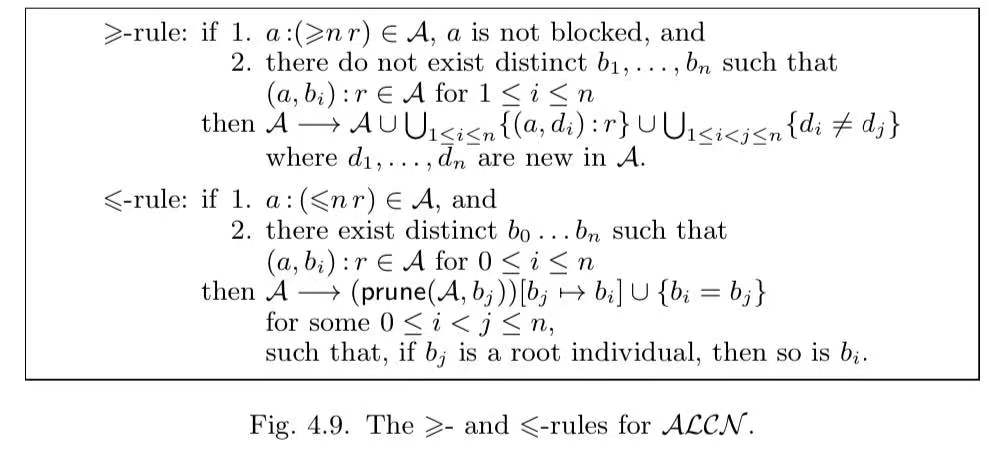
\includegraphics[width=1\textwidth]{2.png}\\
        \caption{ALCN added rules}
        \label{fig:ALCN added rules}
    \end{figure} 
    All the rules explanation is the same as the book.\\
    \textbf{Soundness:}\\
    The proof of soundness is similar to lemma 4.11, but here we need to mention that if we incluede the rule of $\geqslant-rule$,there might be a clash
    if there exist x,y all the child of a,a is blocked, so the rule might not satisfiable.So we construct A'' by this form through A',if a is blocked, we construct the same number of
    individual to fit the restriction of $\geqslant-rule$,so we could create the new individual like xz with the same relation to fit the restriction.This will supplement the merge part of individual.
    So this operation avoid the clash, so with lemma 2.4 ,A'' also complete and clash free.For the rule 2, merge doesn't make a sence,because the A' already complete and clash free.\\
    Also for the interpretation, all of these operation are in the domain and there are no emptyset.\\
    \textbf{Completeness:}\\
    We need to prove the completeness for the two rules.For the 1 rule,if there must do the $\geqslant-rule$,then the $a:(\geqslant nr)$,so $a^I \in (\geqslant nr)^I$, so there at least one A'$\in exp(A,\geqslant-rule,a:(\geqslant nr)) consistent$\\
    For the rule 2, it with the $\sqcup-rule$ are both non-determined.So just do expand if there exist one situation that fit for this two rule.We could the prove that: for the $\sqcup-rule$,there is $a^I \in C^I\ or\ a^I\in D^I$, so at least one A'$\in exp(A,\sqcup-rule,a:C\sqcup D)$ consistent.The same way holds for rule 2. So proved.\\ 

    \section{Question 10}
    We extend the Tableau algorithm from $\mathcal{ALCN}$ to $\mathcal{ALCQ}$ by modifying the $\geq$-rule and the $\leq$-rule as follows:
    \begin{itemize}
        \item[-] For the knowledge base
        \[(\{C\sqsubseteq E\}, \{a:{\leq}{1r}.(D\sqcap E), (a, b) : r, b : C\sqcap D, (a, c) : r, c: D\sqcap E, c : \neg C\}),\]determine whether it is consistent, and whether the proposed algorithm detects this.
    \end{itemize}
    \textbf{Here is the answer:}\\
    First, we simplify the Abox with expansion rules:\\
    cap rule:\\
    \[
        \{ (a, b):r,(a, c) : r, a:{\leq}{1r}.(D\sqcap E), b : C, b: D, c:\neg C,c:D,c:E\}
    \]
    then the $\leqslant-rule$,we could find the only c is satisfiable for $D,E$:\\
    Then we add the Tbox:\\
    \[
        C \sqsubseteq E = \top \sqsubseteq E\sqcup\neg C
    \]
    Then we use the inclusion rule:\\
    \[
        b:E\sqcup \neg C   
    \]
    if $b:\neg C$,then clash, so $b:E$\\
    So the abox:\\
    \[
        \{ (a, b):r,(a, c) : r, a:{\leq}{1r}.(D\sqcap E), b : C, b: D,b:E, c:\neg C,c:D,c:E\}
    \]
    Then here we don't have clash which is fit for the $\leqslant$-rule 
    So we have Abox:\\
    \[
        \{ (a, b):r,(a, c) : r, a:{\leq}{1r}.(D\sqcap E), b : C, b: D,b:E, c:\neg C,c:D,c:E\}
    \]
    This box is inconsistent.\\

    \section{Bouns Question 11}
    The DL $\mathcal{S}$ extends ALC with \emph{transitivity axioms} $\textsf{trans}(r)$ for role names $r\in\textsf{R}$. Their semantics is defined as follows: $\mathcal{I}\models\textsf{trans}(r)$ iff $r^{\mathcal{I}}$ is transitive. Furthermore, an $\mathcal{S}$ knowledge base $\mathcal{K}:=(\mathcal{T}, \mathcal{A}, \mathcal{R})$ consists of an ALC knowledge base $(\mathcal{T}, \mathcal{A})$, and an additional RBox $\mathcal{R}$ of transitivity axioms. Prove the following:
    \begin{itemize}
        \item[-] For an arbitrary TBox $\mathcal{T}$, the concept $C_{\mathcal{T}}$ is defined as $\underset{C\sqsubseteq D\in\mathcal{T}}{\bigsqcup}\neg C\sqcup D$. Then $\mathcal{T}$ and $\mathcal{T}^{\prime}=\{\top\sqsubseteq C_{\mathcal{T}}\}$ have the same models.
        \item[-] Let $\mathcal{K}:=\{\mathcal{T}, \mathcal{A}, \mathcal{R}\}$ be a knowledge base such that, without loss of generality, $\mathcal{T}$ consists of a single GCI $\top\sqsubseteq C_{\mathcal{T}}$, and $C_{\mathcal{T}}$ is in NNF. Define the ALC knowledge base $\mathcal{K}^{+}:=(\mathcal{T}^{+}, \mathcal{A})$ where
        \begin{align*}
            &\mathcal{T}^{+}:=\mathcal{T}\cup\{\forall r.C\sqsubseteq\forall r.\forall r.C~|~\textsf{trans}(r)\in\mathcal{R}~\text{and}~\forall r.C\in\textsf{Sub}(C_{\mathcal{T}})\cup \textsf{Sub}(A)\}.
        \end{align*}
        Then $\mathcal{K}$ is consistent, if and only if, $\mathcal{K}^{+}$ is consistent. Consequently, the Tableau algorithm for ALC can also be used for $\mathcal{S}$.
    \end{itemize}
    \textbf{Here is the answer:}\\
    (1).Prove the $T\ and\ T'$ have the same model:\\
    according to the lemma 2.16(v) we get that:$\mathcal{T}\models C \sqsubseteq D$ if and only if $\mathcal{T}\models T \sqsubseteq (\neg C \sqcup D)$.So we could without loss the generality get that
    the for all inclusions in Tbox $\mathcal{T}$, we have $\underset{C\sqsubseteq D\in\mathcal{T}}{\bigsqcup}\neg C\sqcup D$. So there is also a equivlence that $T \sqsubseteq C_T$, so they are the same, so we could prove that they have the same model.\\
    
    (2).Prove the $\mathcal{K}$ is consistent, if and only if, $\mathcal{K}^{+}$:\\
    $\rightarrow$:\\
    S knowledge base K consists of the KB,this means the model of K is the model of KB.The knowledge base $K^+$ is also a special KB,
    so the model of K is also the mode of $K^+$,so we have if K is consistent, the $K^+$ is consistent according to the lemma 2.4\\
    $\leftarrow$:\\
    The $K^+$ said it is contains with ($T^+$,K):\\
    \[
        \mathcal{T}^{+}:=\mathcal{T}\cup\{\forall r.C\sqsubseteq\forall r.\forall r.C~|~\textsf{trans}(r)\in\mathcal{R}~\text{and}~\forall r.C\in\textsf{Sub}(C_{\mathcal{T}})\cup \textsf{Sub}(A)\}.
    \]
    It means the $Sub(C_T)$ come from the domain, we could find that if we do two times of operation forall, it has a smaller domain than we do one time of forall,
    but if they have the inclusion relationship,this means there must be transition of r so the range of the C will fit the rule of $T^+$,we also could use the Tableau 
    algorithm, with the operation of blocking, we have that there is no cycle in the C.So the relation r must fit the transitivity.Also for $\forall r.C$ is in the set of $Sub(C_T)$.
    So the C is in the domain of $C_T$,so if $T^+$ is consistent, we could select the rules of r which fit the Tableau algorithm and it must in the domain of K. And all r with relationships,
    so if the $K^+$ is consistent, the K is consistent. 


\end{document}


